% Options for packages loaded elsewhere
\PassOptionsToPackage{unicode}{hyperref}
\PassOptionsToPackage{hyphens}{url}
%
\documentclass[
  11pt,
]{article}
\usepackage{amsmath,amssymb}
\usepackage{iftex}
\ifPDFTeX
  \usepackage[T1]{fontenc}
  \usepackage[utf8]{inputenc}
  \usepackage{textcomp} % provide euro and other symbols
\else % if luatex or xetex
  \usepackage{unicode-math} % this also loads fontspec
  \defaultfontfeatures{Scale=MatchLowercase}
  \defaultfontfeatures[\rmfamily]{Ligatures=TeX,Scale=1}
\fi
\usepackage{lmodern}
\ifPDFTeX\else
  % xetex/luatex font selection
\fi
% Use upquote if available, for straight quotes in verbatim environments
\IfFileExists{upquote.sty}{\usepackage{upquote}}{}
\IfFileExists{microtype.sty}{% use microtype if available
  \usepackage[]{microtype}
  \UseMicrotypeSet[protrusion]{basicmath} % disable protrusion for tt fonts
}{}
\makeatletter
\@ifundefined{KOMAClassName}{% if non-KOMA class
  \IfFileExists{parskip.sty}{%
    \usepackage{parskip}
  }{% else
    \setlength{\parindent}{0pt}
    \setlength{\parskip}{6pt plus 2pt minus 1pt}}
}{% if KOMA class
  \KOMAoptions{parskip=half}}
\makeatother
\usepackage{xcolor}
\usepackage[margin=2.5cm]{geometry}
\usepackage{color}
\usepackage{fancyvrb}
\newcommand{\VerbBar}{|}
\newcommand{\VERB}{\Verb[commandchars=\\\{\}]}
\DefineVerbatimEnvironment{Highlighting}{Verbatim}{commandchars=\\\{\}}
% Add ',fontsize=\small' for more characters per line
\usepackage{framed}
\definecolor{shadecolor}{RGB}{248,248,248}
\newenvironment{Shaded}{\begin{snugshade}}{\end{snugshade}}
\newcommand{\AlertTok}[1]{\textcolor[rgb]{0.94,0.16,0.16}{#1}}
\newcommand{\AnnotationTok}[1]{\textcolor[rgb]{0.56,0.35,0.01}{\textbf{\textit{#1}}}}
\newcommand{\AttributeTok}[1]{\textcolor[rgb]{0.13,0.29,0.53}{#1}}
\newcommand{\BaseNTok}[1]{\textcolor[rgb]{0.00,0.00,0.81}{#1}}
\newcommand{\BuiltInTok}[1]{#1}
\newcommand{\CharTok}[1]{\textcolor[rgb]{0.31,0.60,0.02}{#1}}
\newcommand{\CommentTok}[1]{\textcolor[rgb]{0.56,0.35,0.01}{\textit{#1}}}
\newcommand{\CommentVarTok}[1]{\textcolor[rgb]{0.56,0.35,0.01}{\textbf{\textit{#1}}}}
\newcommand{\ConstantTok}[1]{\textcolor[rgb]{0.56,0.35,0.01}{#1}}
\newcommand{\ControlFlowTok}[1]{\textcolor[rgb]{0.13,0.29,0.53}{\textbf{#1}}}
\newcommand{\DataTypeTok}[1]{\textcolor[rgb]{0.13,0.29,0.53}{#1}}
\newcommand{\DecValTok}[1]{\textcolor[rgb]{0.00,0.00,0.81}{#1}}
\newcommand{\DocumentationTok}[1]{\textcolor[rgb]{0.56,0.35,0.01}{\textbf{\textit{#1}}}}
\newcommand{\ErrorTok}[1]{\textcolor[rgb]{0.64,0.00,0.00}{\textbf{#1}}}
\newcommand{\ExtensionTok}[1]{#1}
\newcommand{\FloatTok}[1]{\textcolor[rgb]{0.00,0.00,0.81}{#1}}
\newcommand{\FunctionTok}[1]{\textcolor[rgb]{0.13,0.29,0.53}{\textbf{#1}}}
\newcommand{\ImportTok}[1]{#1}
\newcommand{\InformationTok}[1]{\textcolor[rgb]{0.56,0.35,0.01}{\textbf{\textit{#1}}}}
\newcommand{\KeywordTok}[1]{\textcolor[rgb]{0.13,0.29,0.53}{\textbf{#1}}}
\newcommand{\NormalTok}[1]{#1}
\newcommand{\OperatorTok}[1]{\textcolor[rgb]{0.81,0.36,0.00}{\textbf{#1}}}
\newcommand{\OtherTok}[1]{\textcolor[rgb]{0.56,0.35,0.01}{#1}}
\newcommand{\PreprocessorTok}[1]{\textcolor[rgb]{0.56,0.35,0.01}{\textit{#1}}}
\newcommand{\RegionMarkerTok}[1]{#1}
\newcommand{\SpecialCharTok}[1]{\textcolor[rgb]{0.81,0.36,0.00}{\textbf{#1}}}
\newcommand{\SpecialStringTok}[1]{\textcolor[rgb]{0.31,0.60,0.02}{#1}}
\newcommand{\StringTok}[1]{\textcolor[rgb]{0.31,0.60,0.02}{#1}}
\newcommand{\VariableTok}[1]{\textcolor[rgb]{0.00,0.00,0.00}{#1}}
\newcommand{\VerbatimStringTok}[1]{\textcolor[rgb]{0.31,0.60,0.02}{#1}}
\newcommand{\WarningTok}[1]{\textcolor[rgb]{0.56,0.35,0.01}{\textbf{\textit{#1}}}}
\usepackage{graphicx}
\makeatletter
\def\maxwidth{\ifdim\Gin@nat@width>\linewidth\linewidth\else\Gin@nat@width\fi}
\def\maxheight{\ifdim\Gin@nat@height>\textheight\textheight\else\Gin@nat@height\fi}
\makeatother
% Scale images if necessary, so that they will not overflow the page
% margins by default, and it is still possible to overwrite the defaults
% using explicit options in \includegraphics[width, height, ...]{}
\setkeys{Gin}{width=\maxwidth,height=\maxheight,keepaspectratio}
% Set default figure placement to htbp
\makeatletter
\def\fps@figure{htbp}
\makeatother
\setlength{\emergencystretch}{3em} % prevent overfull lines
\providecommand{\tightlist}{%
  \setlength{\itemsep}{0pt}\setlength{\parskip}{0pt}}
\setcounter{secnumdepth}{5}
\usepackage{graphicx}
\usepackage{amsmath}
\usepackage{booktabs}
\usepackage{caption}
\usepackage{fancyhdr}
\usepackage{ragged2e}
\usepackage{multicol}
\justifying
\pagestyle{fancy}
\fancyhead[L]{Clara Delandre, Majandra Garcia, Paola Biocchi, Coline Leteurte}
\fancyfoot[C]{\thepage}
\usepackage{booktabs}
\usepackage{longtable}
\usepackage{array}
\usepackage{multirow}
\usepackage{wrapfig}
\usepackage{float}
\usepackage{colortbl}
\usepackage{pdflscape}
\usepackage{tabu}
\usepackage{threeparttable}
\usepackage{threeparttablex}
\usepackage[normalem]{ulem}
\usepackage{makecell}
\usepackage{xcolor}
\ifLuaTeX
  \usepackage{selnolig}  % disable illegal ligatures
\fi
\usepackage{bookmark}
\IfFileExists{xurl.sty}{\usepackage{xurl}}{} % add URL line breaks if available
\urlstyle{same}
\hypersetup{
  pdftitle={Predicting Mortgage Yield using Regression Analysis},
  pdfauthor={Group 42},
  hidelinks,
  pdfcreator={LaTeX via pandoc}}

\title{Predicting Mortgage Yield using Regression Analysis}
\author{Group 42}
\date{2025-04-01}

\begin{document}
\maketitle

\section{Introduction}\label{introduction}

The study of A. H. Schaaf, 1966, ``Regional Differences in Mortgage
Financing Costs'' investigates the existence and causes of regional
differences in mortgage financing costs in the United States. These
differences in mortgage yields have decreased in the early 20th century,
however they remained stable after World War 2. The paper explores two
main explanations for this phenomenon:\\
\strut \\
\textbf{1.} differences in investment value due to risk, terms, and
liquidity\\
\textbf{2.} market imperfections such as legal barriers and information
gaps.\\
\strut \\
The data used in this study comes from the Federal Home Loan Bank Board,
which contains interest rates and fees in 18 SMSAs (Standard
Metropolitan Statistical Areas). The findings suggest that distance from
major financial centers, risk levels, and local demand for savings
significantly affect mortgage yields. However, market structure and
overall savings levels play a lesser role.\\
\strut \\
The aim of this report is to analyze the data and develop a predictive
model to predict Mortgage Yield (\texttt{mortYld}) based on 8
explanatory variables:\\
\strut \\
- \textbf{smsa:} Standard Metropolitan Statistical Areas (18) → Name of
the city/region.\\
- \textbf{mortYld:} Mortgage Yield, in \% → The percentage return on a
mortgage.\\
- \textbf{X1:} Loan-to-Mortgage Ratio, in \% → High values indicate low
down payments.\\
- \textbf{X2:} Distance from Boston, in miles → Measures regional
proximity to financial centers.\\
- \textbf{X3:} Savings per new unit built, in \$ → Indicator of regional
credit demand.\\
- \textbf{X4:} Savings per capita, in \$ → Measures local savings levels
(credit supply).\\
- \textbf{X5:} Population increase, 1950-1960, in \% → Proxy for housing
demand growth.\\
- \textbf{X6:} Percentage of first mortgages from inter-regional banks,
in \% → Indicator of external financing reliance.\\

\begin{center}\rule{0.5\linewidth}{0.5pt}\end{center}

\section{Exploratory Data Analysis
(EDA)}\label{exploratory-data-analysis-eda}

\subsection{Load Data and Libraries}\label{load-data-and-libraries}

\begin{longtable}[t]{lrrrrrrr}
\caption{\label{tab:unnamed-chunk-1}First few rows of the dataset}\\
\toprule
smsa & mortYld & X1 & X2 & X3 & X4 & X5 & X6\\
\midrule
Los Angeles-Long Bea & 6.17 & 78.1 & 3042 & 91.3 & 1738.1 & 45.5 & 33.1\\
Denver & 6.06 & 77.0 & 1997 & 84.1 & 1110.4 & 51.8 & 21.9\\
San Francisco-Oaklan & 6.04 & 75.7 & 3162 & 129.3 & 1738.1 & 24.0 & 46.0\\
Dallas-Fort Worth & 6.04 & 77.4 & 1821 & 41.2 & 778.4 & 45.7 & 51.3\\
Miami & 6.02 & 77.4 & 1542 & 119.1 & 1136.7 & 88.9 & 18.7\\
\addlinespace
Atlanta & 6.02 & 73.6 & 1074 & 32.3 & 582.9 & 39.9 & 26.6\\
\bottomrule
\end{longtable}

\begin{verbatim}
##    smsa mortYld      X1      X2      X3      X4      X5      X6 
##       0       0       0       0       0       0       0       0
\end{verbatim}

Here is a display of the data, on the first few rows of the dataset. It
contains mortgage yield (mortYld) as the dependent variable and six
variables (X1 to X6). smsa represents the Standard Metropolitan
Statistical Area which is the name of the city/region. We can observe
that all data are numerical values and there is no missing value for
each region.

\subsection{Univariate Analysis}\label{univariate-analysis}

\subsubsection{Summary Statistics}\label{summary-statistics}

\begin{longtable}[t]{llllllll}
\caption{\label{tab:unnamed-chunk-3}Summary Statistics of Variables}\\
\toprule
 & mortYld & X1 & X2 & X3 & X4 & X5 & X6\\
\midrule
 & Min.   :5.280 & Min.   :67.00 & Min.   :   0 & Min.   : 32.3 & Min.   : 582.9 & Min.   : 7.50 & Min.   : 2.00\\
 & 1st Qu.:5.678 & 1st Qu.:70.03 & 1st Qu.: 648 & 1st Qu.: 85.9 & 1st Qu.: 792.9 & 1st Qu.:23.18 & 1st Qu.: 9.55\\
 & Median :5.880 & Median :73.25 & Median :1364 & Median :122.2 & Median :1161.3 & Median :27.35 & Median :18.70\\
 & Mean   :5.841 & Mean   :73.38 & Mean   :1389 & Mean   :159.8 & Mean   :1245.9 & Mean   :33.03 & Mean   :20.95\\
 & 3rd Qu.:6.020 & 3rd Qu.:77.22 & 3rd Qu.:1847 & 3rd Qu.:218.2 & 3rd Qu.:1556.6 & 3rd Qu.:44.10 & 3rd Qu.:30.43\\
\addlinespace
 & Max.   :6.170 & Max.   :78.10 & Max.   :3162 & Max.   :428.2 & Max.   :2582.4 & Max.   :88.90 & Max.   :51.30\\
\bottomrule
\end{longtable}

We can observe that each variable 18 observations corresponding to 18
different SMSAs. Through this summary, we can already observe mortgage
yields don't vary much across regions. Most values are between 5.5\% and
6.2\%, suggesting relatively stable mortgage rates.

Loan-to-mortgage ratios (X1) are concentrated in between 70\% and 78\%,
with low variance. Savings per New Unit Built (X3) are characterized by
a mean bigger than the median, representing a right-skewed distribution
and then large disparities in housing affordability across regions.

-\textgreater{} to complete

\subsubsection{Graphical Representation}\label{graphical-representation}

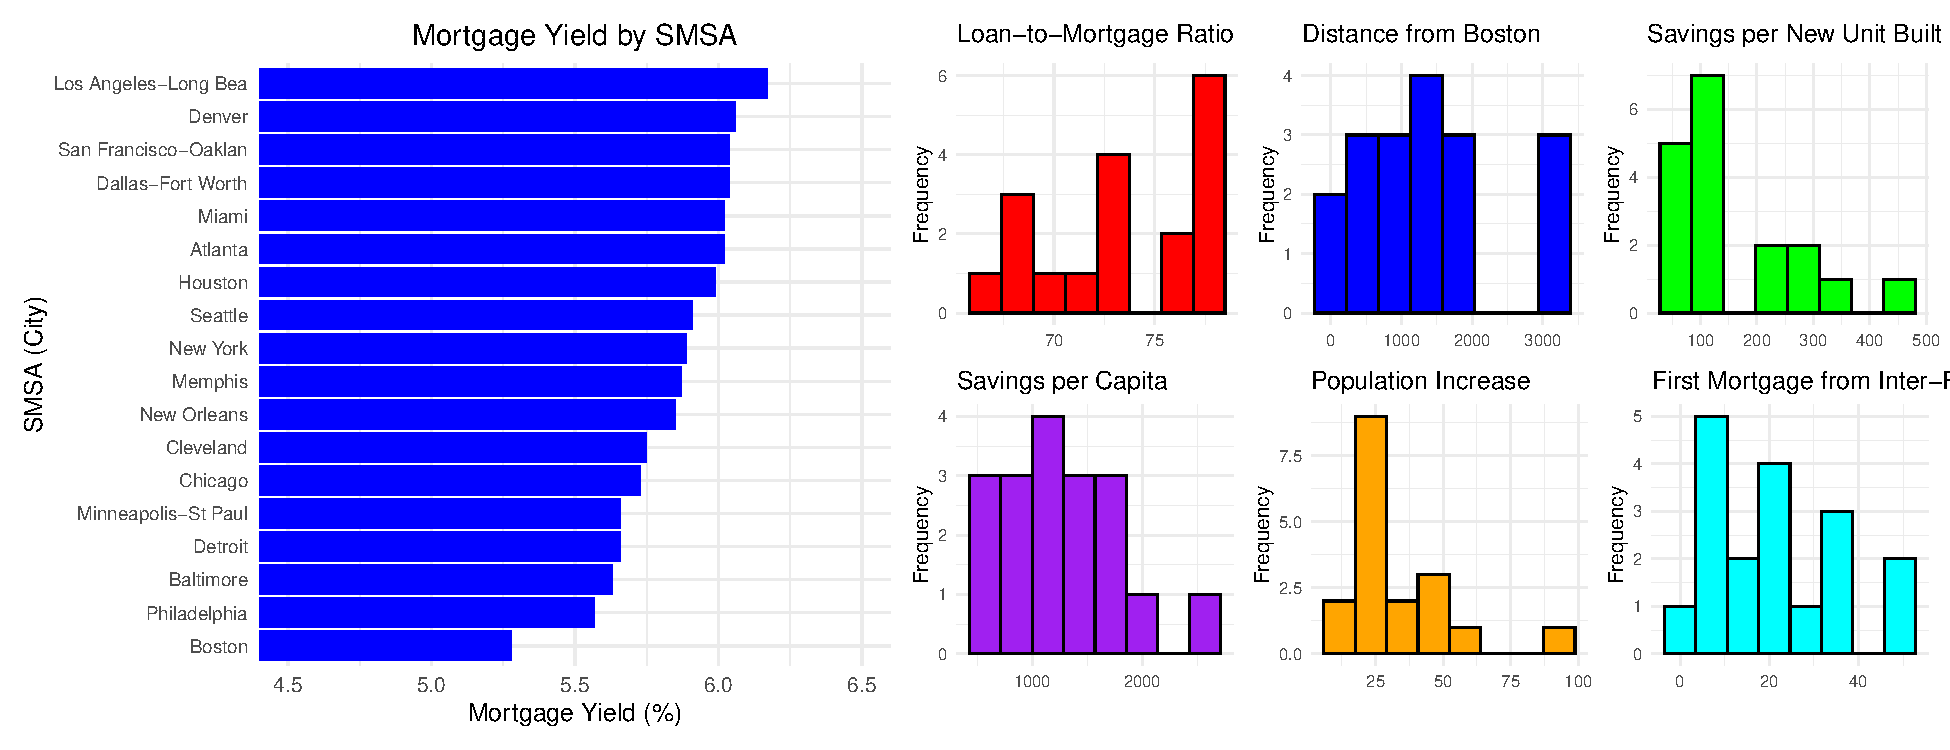
\includegraphics{Figs/unnamed-chunk-4-1.pdf}

There is not a huge variation in mortgage yield across SMSAs, as most
bars are at similar heights but if we focus in between 4 and 6\%, we see
regional differences exist in mortgage yields, possibly due to economic
factors like savings, loan terms, and regional banking practices.

The histograms reveal the characteristics of the predictor variables.

The loan-to-mortgage ratio (X1) shows low variance with most values
concentrated between 66\% and 80\%, possibly indicating limited
variability across regions.

Distance from Boston (X2) displays a wide distribution, reflecting
substantial geographic spread among SMSAs.

Savings per new unit built (X3) and savings per capita (X4) both exhibit
right-skewed distributions, suggesting that a few cities have notably
higher savings levels.

Population increase (X5) is also highly skewed with one major outlier,
indicating that most cities had moderate growth, while a few experienced
rapid expansion.

Finally, the percentage of first mortgages from inter-regional banks
(X6) is also right-skewed, with most cities relying minimally on
external financing and a few showing heavy dependence.

These patterns suggest that certain variables may benefit from
transformation prior to regression modeling.

\subsection{Bivariate Numerical
Analysis}\label{bivariate-numerical-analysis}

\subsubsection{Association Analysis}\label{association-analysis}

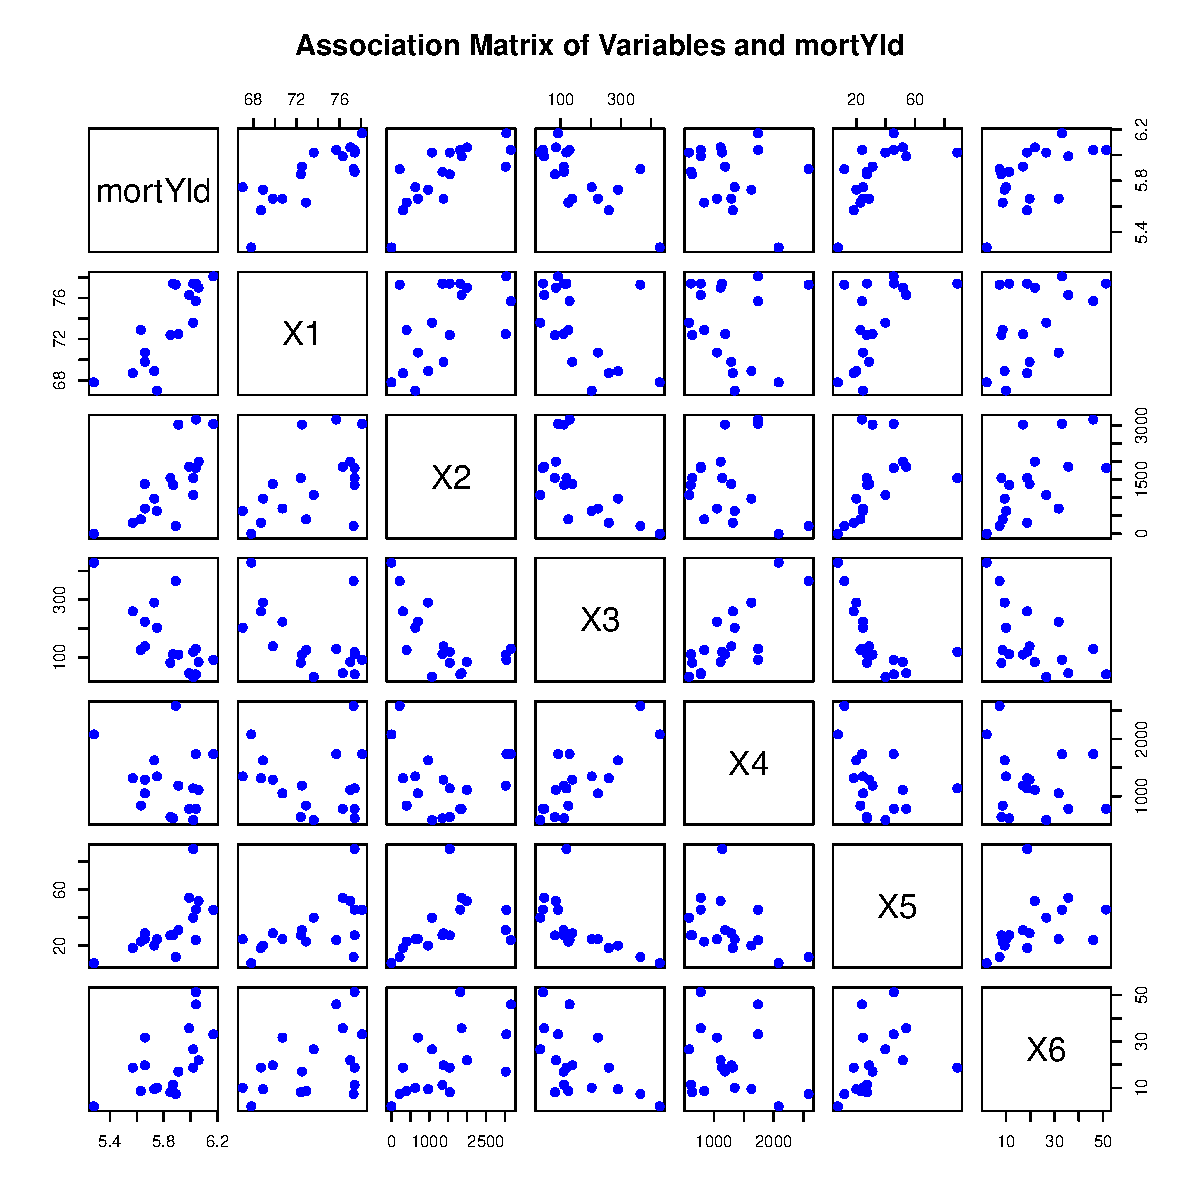
\includegraphics{Figs/unnamed-chunk-5-1.pdf}

The scatterplot matrix provides a quick visual assessment of linearity,
strength of associations among predictors, and outlier detection. It
complements numerical analyses like the correlation matrix and VIF.

We can visualizes bivariate relationships, how each variable relates to
the others, especially to mortYld and assess if a relationship is
linear, curved, or weak, positive or negative. We can also spot outliers
or cities that don't follow the general trend.

We can see that most of the plots are random dispersion, some are
linear, and some are curved. X3 seems to be positively associated with
X4 and negatively with X5. X2 and X3 seem exponentially associated.
mortYld and X5 seem to be associated in a squared root maner.

Let's take a closer look into the Association Matrix, regarding the
relationship between Mortgage Yield (\%) and the explanatory variables
(x-axis), representing the first column in the precedent figure.

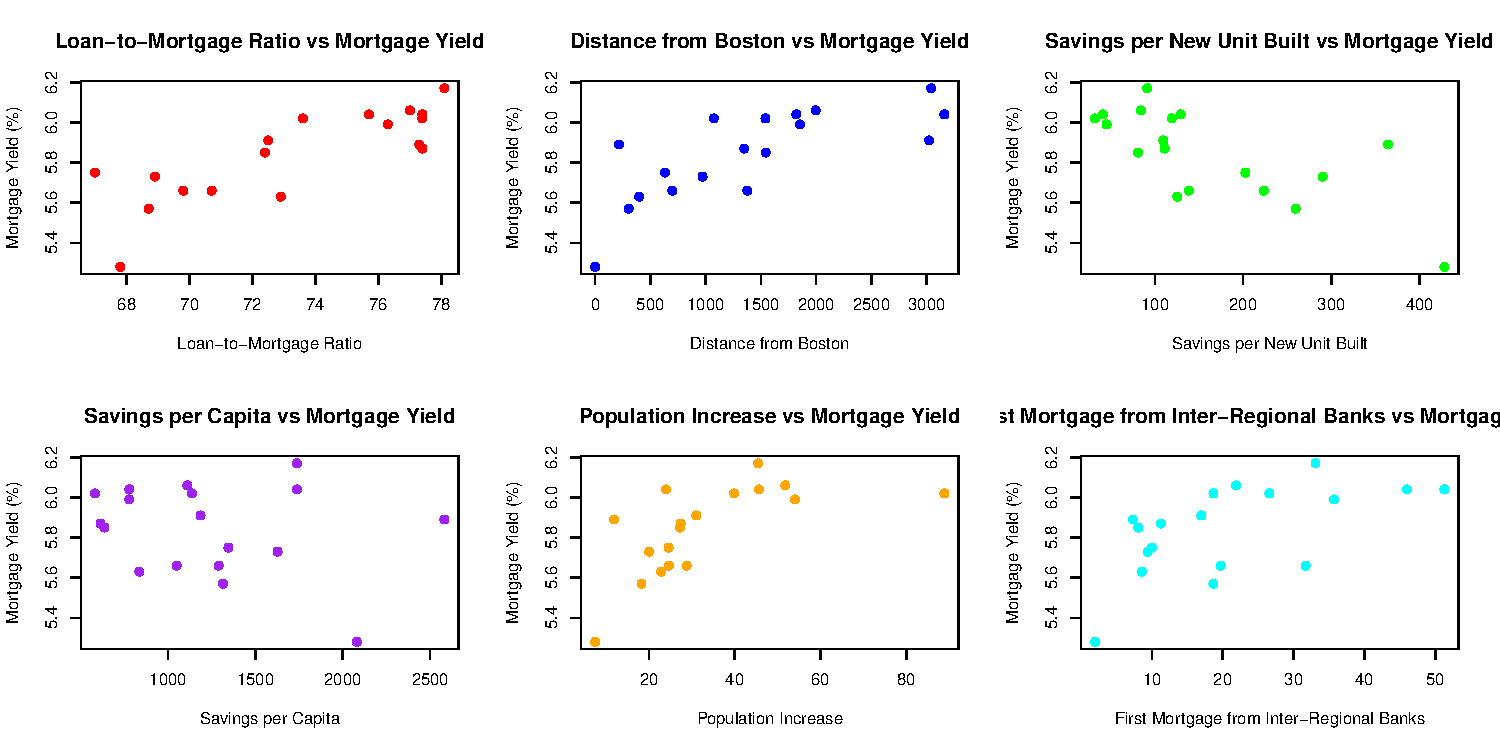
\includegraphics{Figs/unnamed-chunk-6-1.pdf}

\textbf{1. Loan-to-Mortgage Ratio:} As this ratio increases, the
Mortgage Yield increases. This suggests a positive correlation, and that
higher loan-to-mortgage ratios (more borrowed money relative to the
property value) are associated with higher mortgage yields.\\
\textbf{2. Distance from Boston:} There is a positive correlation.
Boston represents a major financial center with surplus capital. Regions
further from Boston might have higher yields.\\
\textbf{3. Savings per New Unit Built :} There is a negative
correlation. This indicates that areas with more savings dedicated to
new construction have better access to local financing, resulting in
lower mortgage yields.\\
\textbf{4. Savings per Capita:} The relationship is less clear but
appears to be a weak negative correlation or a random dispersion.\\
\textbf{5. Population Increase:} There is a positive association which
can be seen as a square-root relationship. High population growth may
imply higher demand for housing, increasing mortgage yields due to
heightened competition for available funds. We can observe a potential
outlier at the right side of the plot.\\
\textbf{6. First Mortgage from Inter-Regional Banks:} No clear trend. It
seems like the reliance on external financing (measured by the
percentage of first mortgages from inter-regional banks) does not
significantly influence mortgage yields.\\
\strut \\
\textbf{To resume:}\\
- X1, X2 and X5 seem to be the most influential variables positively
correlated with Mortgage Yield.\\
- X3 is the most influential negative variable.\\
- X4 X6 variables show weak relationships with mortgage yields.\\
- These observations support the findings of Schaaf (1966) that distance
from financial centers, risk factors, and local demand for savings
contribute to yield variations.\\

\subsubsection{Correlation analysis}\label{correlation-analysis}

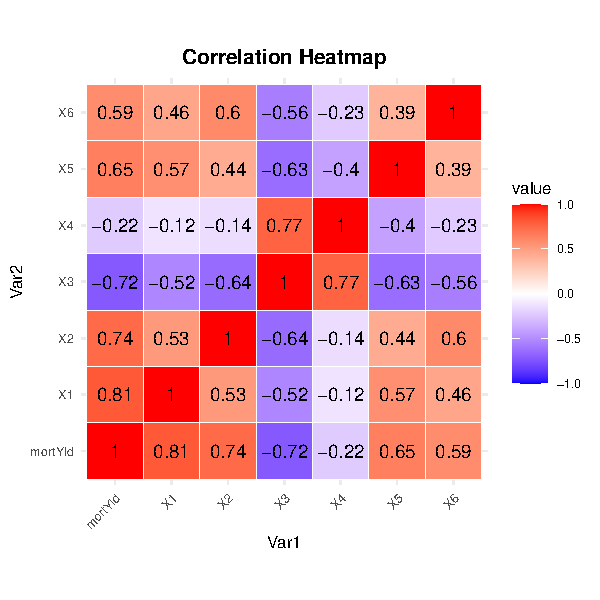
\includegraphics{Figs/unnamed-chunk-7-1.pdf}

X3 and X4 are strongly correlated (0.77).

X2 and X3 have a high negative correlation (-0.64).

X3 is also strongly negatively correlated with X5 at -0.63.

X1, X2 and X5 have a high positive correlation with mortYld, and X3 a
strong negative one. In consequence, we can confirm our previous
statements about the scatter-plots.

We can then think about removing one of the highly correlated
predictors, if multicollinearity affects the regression model.

These correlations tell only about the if the variables are linearly
associated. A low value doesn't mean that the variables are not
correlated in another way.

\begin{Shaded}
\begin{Highlighting}[]
\FunctionTok{cor}\NormalTok{(}\FunctionTok{residuals}\NormalTok{(}\FunctionTok{lm}\NormalTok{(df}\SpecialCharTok{$}\NormalTok{X2 }\SpecialCharTok{\textasciitilde{}}\NormalTok{ df}\SpecialCharTok{$}\NormalTok{X3)), }\FunctionTok{residuals}\NormalTok{(}\FunctionTok{lm}\NormalTok{(df}\SpecialCharTok{$}\NormalTok{X6 }\SpecialCharTok{\textasciitilde{}}\NormalTok{ df}\SpecialCharTok{$}\NormalTok{X3)))}
\end{Highlighting}
\end{Shaded}

\begin{verbatim}
## [1] 0.3760938
\end{verbatim}

We can also see that X2 is only weakly positively correlated (r = 0.21)
to X6 after controlling for X3; compare this to the much higher simple
correlation (r = 0.60). In other words, much of the apparent correlation
between X2 and X6 can be explained by their mutual positive correlation
with X3.

\begin{center}\rule{0.5\linewidth}{0.5pt}\end{center}

\section{Model Fitting}\label{model-fitting}

In this analysis, all predictors are continuous variables and each
observation corresponds to a unique SMSA. Since the dataset contains no
grouping or categorical factors with unequal group sizes, this is a
standard multiple regression model with one observation per row.
Therefore, the design is not factorial and does not involve unbalanced
group structures. As a result, the order in which predictors are entered
into the lm() function does not influence the coefficient estimates,
F-tests, or model interpretation.

\subsection{Pairwise Simple
Regressions}\label{pairwise-simple-regressions}

\begin{longtable}[t]{lrr}
\caption{\label{tab:unnamed-chunk-9}Simple Linear Regressions: R² and p-values}\\
\toprule
Predictor & R\_squared & p\_value\\
\midrule
X1 & 0.654 & 0.0000\\
X2 & 0.546 & 0.0005\\
X3 & 0.517 & 0.0008\\
X4 & 0.049 & 0.3763\\
X5 & 0.419 & 0.0037\\
\addlinespace
X6 & 0.346 & 0.0103\\
\bottomrule
\end{longtable}

The table summarizes the strength of individual linear relationships
between each predictor (X1--X6) and the mortgage yield using simple
linear regression.

\begin{verbatim}
•   **X1** has the **strongest linear association** with mortgage yield,
\end{verbatim}

explaining approximately \textbf{65.4\% of its variance} and is highly
significant (p \textless{} 0.001)

\begin{verbatim}
•   **X2** and **X3** also show strong and significant associations (R² =
\end{verbatim}

0.546 and 0.517, respectively).

\begin{verbatim}
•   **X5** and **X6** show moderate yet significant associations (R² =
\end{verbatim}

0.419 and 0.346).

\begin{verbatim}
•   **X4 (Savings per Capita)** does **not** show a significant
\end{verbatim}

relationship with mortgage yield (R² = 0.049, p = 0.3763), suggesting it
may not be a strong individual predictor.

This preliminary analysis indicates that variables X1, X2, and X3 are
the most promising candidates for predicting mortgage yield in a
multivariate model.

\subsection{Null Model vs Full Model
Comparison}\label{null-model-vs-full-model-comparison}

\begin{verbatim}
## Analysis of Variance Table
## 
## Model 1: mortYld ~ 1
## Model 2: mortYld ~ X1 + X2 + X3 + X4 + X5 + X6
##   Res.Df     RSS Df Sum of Sq      F    Pr(>F)    
## 1     17 0.84858                                  
## 2     11 0.10980  6   0.73877 12.335 0.0002523 ***
## ---
## Signif. codes:  0 '***' 0.001 '**' 0.01 '*' 0.05 '.' 0.1 ' ' 1
\end{verbatim}

The ANOVA comparison between the null model and the full model reveals
that the full model, which includes the predictors, significantly
improves the model fit. The null model (intercept-only) does not explain
much of the variation in mortgage yield.

The full model, provides a better explanation of the mortgage yield, as
shown by the significant F-statistic and the p-value. This indicates
that at least one of the predictors is significantly related to mortgage
yield, and the explanatory variables are useful for improving the model.

\begin{verbatim}
## 
## Call:
## lm(formula = mortYld ~ X1 + X2 + X3 + X4 + X5 + X6, data = df)
## 
## Residuals:
##       Min        1Q    Median        3Q       Max 
## -0.145030 -0.017814  0.001474  0.034316  0.134565 
## 
## Coefficients:
##               Estimate Std. Error t value Pr(>|t|)    
## (Intercept)  4.285e+00  6.682e-01   6.413 4.99e-05 ***
## X1           2.033e-02  9.308e-03   2.184   0.0515 .  
## X2           1.359e-05  4.692e-05   0.290   0.7775    
## X3          -1.584e-03  7.532e-04  -2.103   0.0593 .  
## X4           2.017e-04  1.124e-04   1.794   0.1002    
## X5           1.283e-03  1.765e-03   0.727   0.4826    
## X6           2.357e-04  2.302e-03   0.102   0.9203    
## ---
## Signif. codes:  0 '***' 0.001 '**' 0.01 '*' 0.05 '.' 0.1 ' ' 1
## 
## Residual standard error: 0.09991 on 11 degrees of freedom
## Multiple R-squared:  0.8706, Adjusted R-squared:    0.8 
## F-statistic: 12.33 on 6 and 11 DF,  p-value: 0.0002523
\end{verbatim}

The model explains approximately \textbf{87\%} of the variance in
mortgage yield, and after adjusting for the number of predictors,
\textbf{80\%} is still explained. This is a strong fit. The overall
model is statistically significant, with a very low p-value. Once again,
it means that at least one predictor contributes significantly to
explaining the variation in mortYld. The intercept appears to be really
significant to fit the model.

However, most variables do not show statistically significant individual
contributions. Only X1 and X3 show strong significance (p \(\approx\)
0.05). Other variables, X2, X5 and X6, do not show strong individual
effects. This suggests that a reduced model may be more interpretable.

\subsection{Make stepwise regression to select the best
model}\label{make-stepwise-regression-to-select-the-best-model}

\begin{verbatim}
## Start:  AIC=-77.79
## mortYld ~ X1 + X2 + X3 + X4 + X5 + X6
## 
##        Df Sum of Sq     RSS     AIC
## - X6    1  0.000105 0.10991 -79.773
## - X2    1  0.000837 0.11064 -79.653
## - X5    1  0.005271 0.11507 -78.946
## <none>              0.10980 -77.790
## - X4    1  0.032141 0.14194 -75.168
## - X3    1  0.044144 0.15395 -73.707
## - X1    1  0.047593 0.15740 -73.308
## 
## Step:  AIC=-79.77
## mortYld ~ X1 + X2 + X3 + X4 + X5
## 
##        Df Sum of Sq     RSS     AIC
## - X2    1  0.000971 0.11088 -81.614
## - X5    1  0.005259 0.11517 -80.931
## <none>              0.10991 -79.773
## + X6    1  0.000105 0.10980 -77.790
## - X4    1  0.033056 0.14297 -77.040
## - X3    1  0.046942 0.15685 -75.371
## - X1    1  0.048227 0.15813 -75.224
## 
## Step:  AIC=-81.61
## mortYld ~ X1 + X3 + X4 + X5
## 
##        Df Sum of Sq     RSS     AIC
## - X5    1  0.005047 0.11593 -82.813
## <none>              0.11088 -81.614
## + X2    1  0.000971 0.10991 -79.773
## + X6    1  0.000238 0.11064 -79.653
## - X1    1  0.047325 0.15820 -77.216
## - X4    1  0.076985 0.18786 -74.123
## - X3    1  0.139427 0.25031 -68.958
## 
## Step:  AIC=-82.81
## mortYld ~ X1 + X3 + X4
## 
##        Df Sum of Sq     RSS     AIC
## <none>              0.11593 -82.813
## + X5    1  0.005047 0.11088 -81.614
## + X2    1  0.000759 0.11517 -80.931
## + X6    1  0.000202 0.11572 -80.845
## - X1    1  0.065583 0.18151 -76.743
## - X4    1  0.075826 0.19175 -75.755
## - X3    1  0.164703 0.28063 -68.900
\end{verbatim}

\begin{verbatim}
## 
## Call:
## lm(formula = mortYld ~ X1 + X3 + X4, data = df)
## 
## Residuals:
##       Min        1Q    Median        3Q       Max 
## -0.172291 -0.018862  0.006091  0.040552  0.145956 
## 
## Coefficients:
##               Estimate Std. Error t value Pr(>|t|)    
## (Intercept)  4.223e+00  5.814e-01   7.263 4.14e-06 ***
## X1           2.229e-02  7.922e-03   2.814 0.013787 *  
## X3          -1.863e-03  4.178e-04  -4.460 0.000539 ***
## X4           2.249e-04  7.433e-05   3.026 0.009070 ** 
## ---
## Signif. codes:  0 '***' 0.001 '**' 0.01 '*' 0.05 '.' 0.1 ' ' 1
## 
## Residual standard error: 0.091 on 14 degrees of freedom
## Multiple R-squared:  0.8634, Adjusted R-squared:  0.8341 
## F-statistic: 29.49 on 3 and 14 DF,  p-value: 2.618e-06
\end{verbatim}

(mettre en annexe ?)

The stepwise regression process identified X1, X3, and X4 as the most
significant predictors of mortality yield, leading to the final model.

It's interesting to see that X4 appears among the 3 most significant
predictoes although it shows the weakest correlation in the correlation
matrix. Multiple regression measures the effect of each variable while
holding all other constant. As X4 has very strong correlation with X3,
holding X3 can make the unique contribution of X4 clearer.

The final model explains approximately \textbf{83.4\% of the variance}
in mortgage yield using only these three predictors.\\
The AIC isn't increased by a lot when keeping the other variables, which
means that these are still statistically valid but not so useful. The
final is simpler but still explain the data just as well or better.

The residual standard error (0.091) is low, and the overall model is
highly significant, indicating a good fit.\\
We end up with : mortYld = 4.223 + 0.02229.X1 - 0.001863.X3 +
0.0002249.X4\\

Let's try a model with 2-way interactions.

\begin{verbatim}
## 
## Call:
## lm(formula = mortYld ~ X1 + X3 + X4 + X1:X3 + X1:X4 + X3:X4, 
##     data = df)
## 
## Residuals:
##       Min        1Q    Median        3Q       Max 
## -0.187649 -0.015613  0.007221  0.030851  0.155167 
## 
## Coefficients:
##               Estimate Std. Error t value Pr(>|t|)  
## (Intercept)  5.371e+00  2.033e+00   2.642   0.0229 *
## X1           6.912e-03  2.657e-02   0.260   0.7996  
## X3          -1.040e-04  9.611e-03  -0.011   0.9916  
## X4          -9.096e-04  2.454e-03  -0.371   0.7180  
## X1:X3       -2.091e-05  1.322e-04  -0.158   0.8772  
## X1:X4        1.497e-05  3.225e-05   0.464   0.6516  
## X3:X4       -4.751e-08  4.540e-07  -0.105   0.9185  
## ---
## Signif. codes:  0 '***' 0.001 '**' 0.01 '*' 0.05 '.' 0.1 ' ' 1
## 
## Residual standard error: 0.1002 on 11 degrees of freedom
## Multiple R-squared:  0.8698, Adjusted R-squared:  0.7988 
## F-statistic: 12.25 on 6 and 11 DF,  p-value: 0.0002604
\end{verbatim}

The interactions increase the complexity of the model for an improvement
that seems very small.

We decided not to include a 3-way interaction model in our analysis.
Given the small sample size (18 observations), adding high-order
interactions would significantly reduce degrees of freedom and increase
the risk of overfitting. Moreover, 3-way interactions are often
difficult to interpret meaningfully.

\subsection{Model Comparison}\label{model-comparison}

\begin{longtable}[t]{lrrrrr}
\caption{\label{tab:unnamed-chunk-14}Comparison of Model Performance Metrics}\\
\toprule
Model & R2 & Adj\_R2 & AIC & Residual\_SE & F\_statistic\\
\midrule
Full Model & 0.871 & 0.800 & -24.708 & 0.100 & 12.335\\
Stepwise Model & 0.863 & 0.834 & -29.731 & 0.091 & 29.493\\
2-Way Interaction Model & 0.870 & 0.799 & -24.600 & 0.100 & 12.250\\
\bottomrule
\end{longtable}

The \textbf{Stepwise Model} offers the best trade-off between simplicity
and performance: It has the \textbf{lowest AIC}, indicating the best
model fit among the three. Despite having a slightly lower \textbf{R²}
than the full model, it achieves the \textbf{highest Adjusted R²}.

It also has the \textbf{lowest residual standard error} and the
\textbf{highest F-statistic}, confirming overall model significance and
parsimony.

\begin{verbatim}
## Analysis of Variance Table
## 
## Model 1: mortYld ~ X1 + X3 + X4
## Model 2: mortYld ~ X1 + X3 + X4 + X1:X3 + X1:X4 + X3:X4
##   Res.Df     RSS Df Sum of Sq      F Pr(>F)
## 1     14 0.11593                           
## 2     11 0.11046  3 0.0054608 0.1813 0.9069
\end{verbatim}

An ANOVA was conducted to assess whether including 2-way interaction
terms significantly improved the model fit. The test yielded an
F-statistic of 0.18 and a p-value of 0.91, indicating that the
additional interaction terms did not meaningfully reduce the residual
variance.

As a result, we retained the simpler model with only main effects (X1,
X3, and X4), which offers comparable explanatory power and better
interpretability.

\begin{center}\rule{0.5\linewidth}{0.5pt}\end{center}

\section{Model assumptions and
Diagnostics}\label{model-assumptions-and-diagnostics}

\subsection{Independence evaluation}\label{independence-evaluation}

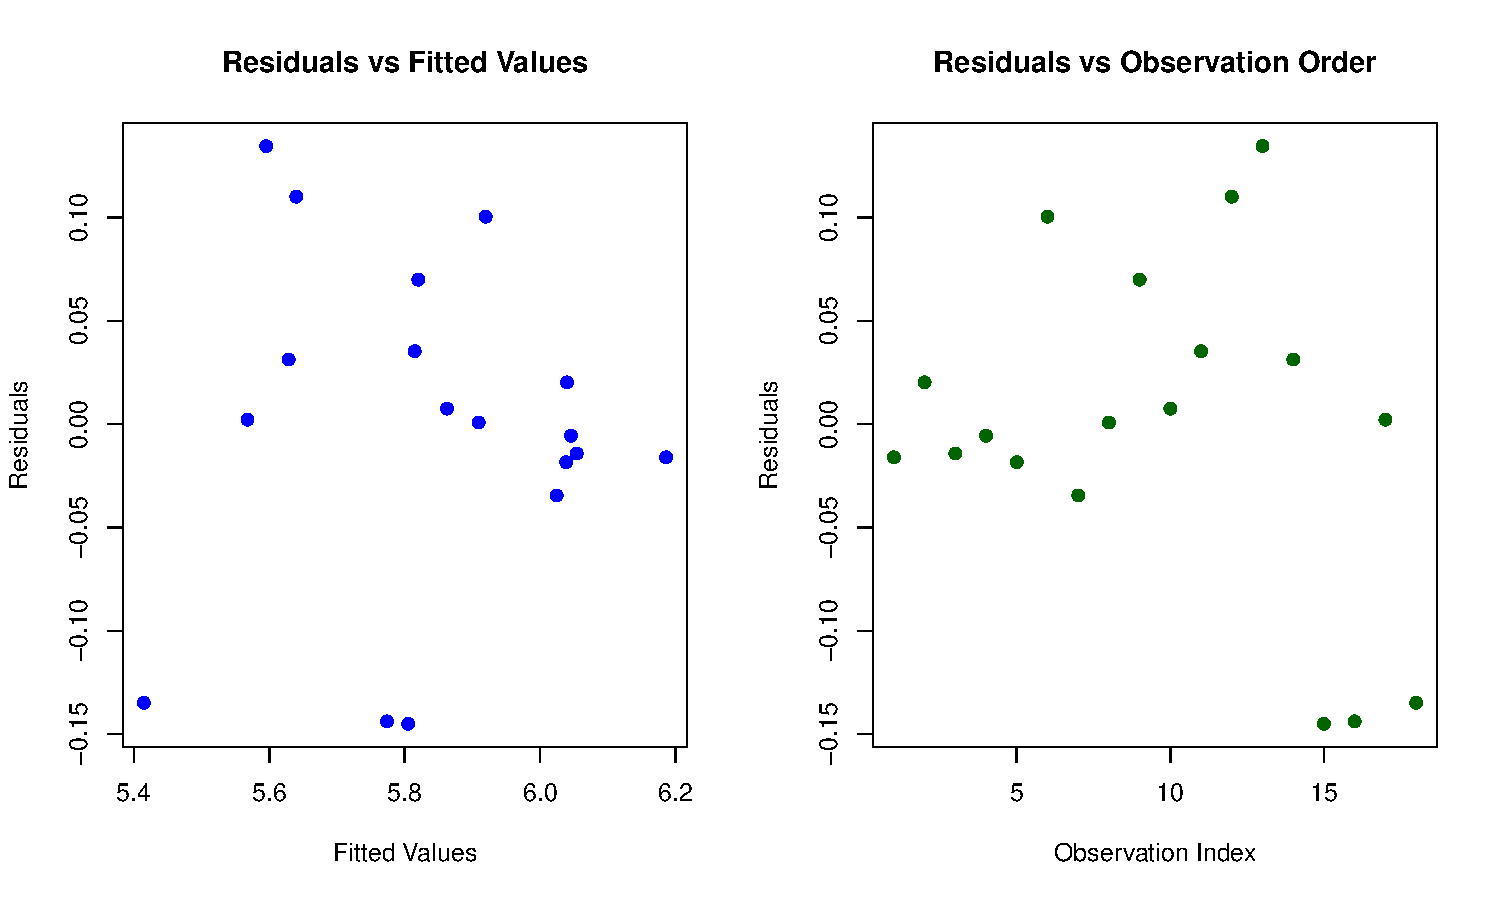
\includegraphics{Figs/unnamed-chunk-16-1.pdf}

The 1st graph shows that the residuals appear randomly scattered around
0. There's no clear pattern. This suggests the assumptions of linearity
and constant error variance (homoscedasticity) are reasonably met.

The 2nd graph can help us conclude that there is no consistent trend so
the independance is verified.

\subsection{Multicolinearity
diagnostic}\label{multicolinearity-diagnostic}

\begin{longtable}[t]{lr}
\caption{\label{tab:unnamed-chunk-17}Variance Inflation Factors (VIF)}\\
\toprule
 & vif\_values\\
\midrule
X1 & 1.886802\\
X3 & 4.550125\\
X4 & 3.348330\\
\bottomrule
\end{longtable}

All variables have a VIF value under 5 meaning that variables are not
too highly related and that no variable should be eliminated. This
confirms our choice of keeping X3 and X4 even if they showed a high
correlation coefficient.

\subsection{Homoscedasticity}\label{homoscedasticity}

Random scatter indicates good assumption of homeoscedasticity. If we can
distinguish a clear pattern, then we have potential heteroscedasticity
issue.

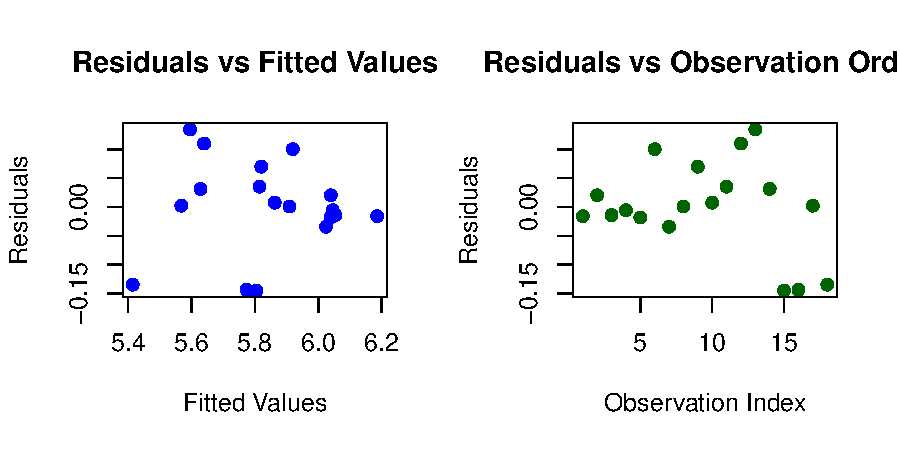
\includegraphics{Figs/unnamed-chunk-18-1.pdf}

\subsection{Normality Check}\label{normality-check}

If points lie on 45 degrees line, it means the residuals are normally
distributed. If we can see a curved pattern, then the normality
assumption is violated

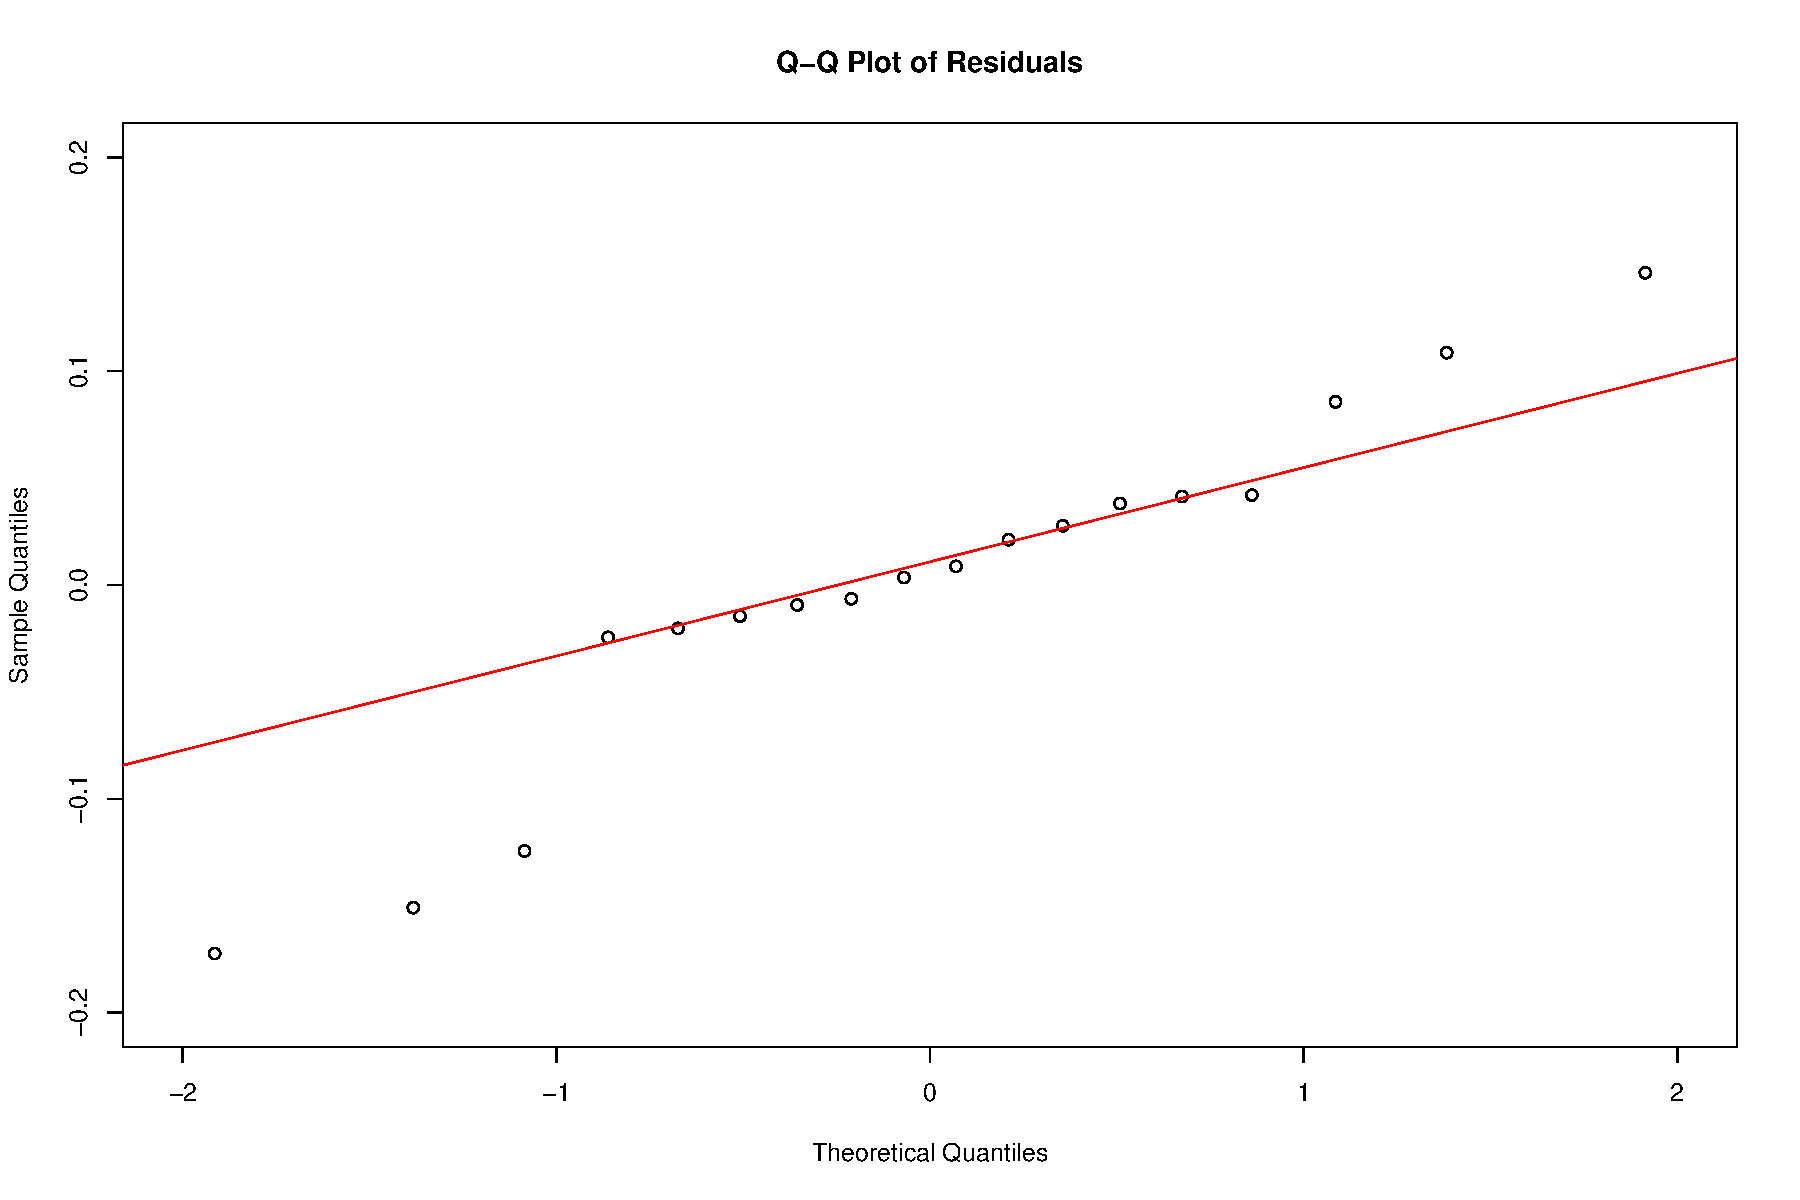
\includegraphics{Figs/unnamed-chunk-19-1.pdf}

\begin{center}\rule{0.5\linewidth}{0.5pt}\end{center}

\section{Final estimated Model}\label{final-estimated-model}

\begin{center}\rule{0.5\linewidth}{0.5pt}\end{center}

\section{Conclusions}\label{conclusions}

\begin{verbatim}
•   The analysis showed that [mention significant predictors] have a strong relationship with mortgage yield.
•   The assumptions of linear regression were [state if met or violated].
•   The model provides [good/poor] predictive accuracy based on [R² and residual analysis].
•   Future improvements could involve [mention possible improvements like transformations, additional predictors, etc.].
\end{verbatim}

\end{document}
